\documentclass[twocolumn]{revtex4}
\usepackage[]{graphicx}
\usepackage{float}
\begin{document}
\title{
Journal article
}
\author{J.~Halle}
\affiliation {Siena College, Loudonville, NY}
\date{November26th2016}
\begin{abstract}
The procedure of doing this problem was somewhat complicated overall. First we got the the google.classroom.com website and download the final project file. For the first problem we establish a function that tests if it rains only 1 day a month. We do this by generating 30 random numbers to represent the days of the month and then we test to see how many times a month it rains. If it rains more then once the we say the occurance of the rain only happening on is false which means that it doesnt count toward the total which is used in finding the percentage. But if it only rains once that month then it goes towards the total of occurances  . then we take the number of occurance in the 100000 and divide it by 100000 and then multiply by 100, and this gives us the percentage of it only raining one time and only one time in a month.
For the 2nd problem we establish a function that tests if it rains 8 or more days in month. We do this by generating 30 random numbers to represent the days of the month and then we test to see how many times a month it rains. If it rains less than 8 days we say the occurance of the rain only happening on is false which means that it doesnt count toward the total which is used in finding the percentage. But if it rains 8 or more days then it goes towards the total of occurances  . then we take the number of occurance in the 100000 and divide it by 100000 and then multiply by 100, and this gives us the percentage of it only raining one time and only one time in a month.
For the 3rd question we create a function to represent the percentage of range amounts. In the function we say that if the probability for the day  is greater then or equal to zero then the probability is 20 percent if not then it runs through the else if statements for the other values. after it runs through the function it returns rain. Then we write a code that test the months to test the probability of it raining atleast 10 cm in one month and inorder to do this we use if and else if statements and use the probabilities provided to calculate how many cm of rain occur that month.
For the next part of 3 we create a histogram of the random data.
For the next part of 3 we are calculating the average amount of rain by taking the total and dividing it by the data that was logged which gives the average
For the final part of question 3 we calculate the uncertainty using numpy functions and "I'm 95 percent confident the rainfall will be between 0 and 21.0"
\end{abstract}
\maketitle
\section{equations}
$$(totalofoccurances/monthstested)*100 =percentage$$

$$averageamountofrain= (totalfromeachmonth/numberofmonths)$$

\section {Histogram Picture}
\begin{figure} [h]
\centering 
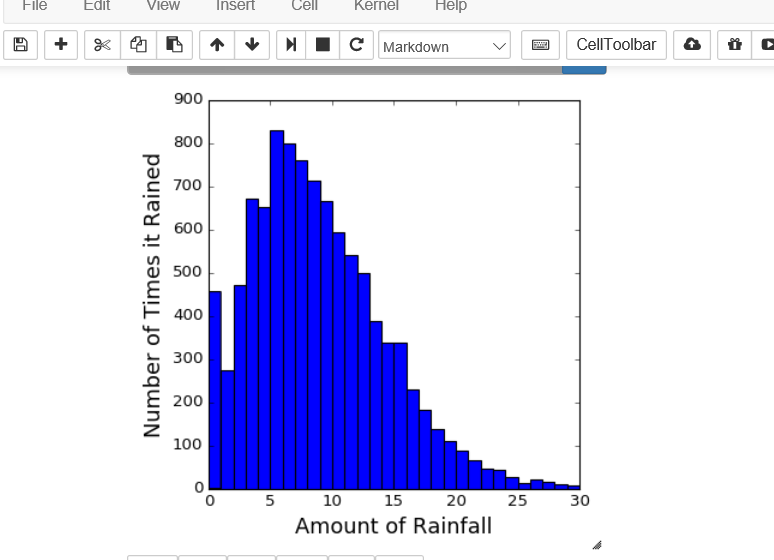
\includegraphics[width=0.5\textwidth] {histogram for final.png}
\caption This is an example of the histograms that could be made with random data.
\end{figure}
\end{document}